\section{Zielsetzung}
Ziel des Franck-Hertz-Versuchs ist es, die Quantennatur der Elektronenhülle von Atomen nachzuweisen. Dafür wird gezeigt, dass 
Quecksilberatome in diskreten Energiespektren Energie aufnehmen, indem Stöße zwischen den Quecksilberatomen und Elektronen 
herbeigeführt werden.

\section{Theorie}
\label{sec:Theorie}
\subsection{Anregung eines Quecksilberatoms}
\label{sec:Anregung}
Damit die Anregungsenergie der Hg-Atome bestimmt werden kann, werden Elektronen mit einer bekannten Energie in Quecksilberdampf 
geschossen. Dabei Stoßen die Elektronen mit den Hg-Atomen zusammen und es kommt sowohl zu unelastischen, als auch zu elastischen 
Stößen.
Die elastischen Stöße sorgen vor allem dafür, dass sich die Geschwindigkeiten und Richtung der Elektronen ändern. Bei den unelastischen
Stößen kommt es hingegen zu einer Erhöhung der Energieniveaus der Hg-Atome.

Durch Detektion der Energie der Elektronen vor und nach den Stößen lässt sich aus der Energiedifferenz die auf das Hg-Atom übertragene
Energie
\begin{equation}
    E_{\symup{a}} = E_1-E_0 = \frac{m_{\symup{e}}v_{\symup{vor}}}{2}-\frac{m_{\symup{e}}v_{\symup{nach}}}{2}
    \label{eq:Anregungsenergie}
\end{equation}
berechnen.

Die von dem Hg-Atom geht nach einer Relaxationszeit von $t\approx\qty{10e-8}{\second}$ in seinen Grundzustand über,
wobei ein Lichtquant mit der Energie
\begin{equation}
    E_{\symup{a}} = hf
    \label{eq:Einstein ist smart}
\end{equation}
emittiert wird.
Für Quecksilber hat diese Energie einen theoretischen Wert von $E_{\symup{a,lit}} = \qty{4,9}{\electronvolt}$.

\subsection{Idealisierte Franck-Hertz-Kurve}
\label{sec:Idealisierte Frank-Hertz-Kurve}
Die Energieniveaus der Hg-Atome lassen sich mit einer Franck-Hertz-Röhre bestimmen,
deren schematischer Aufbau in \autoref{fig:Aufbau} dargestellt ist.
\begin{figure}[H]
    \centering
    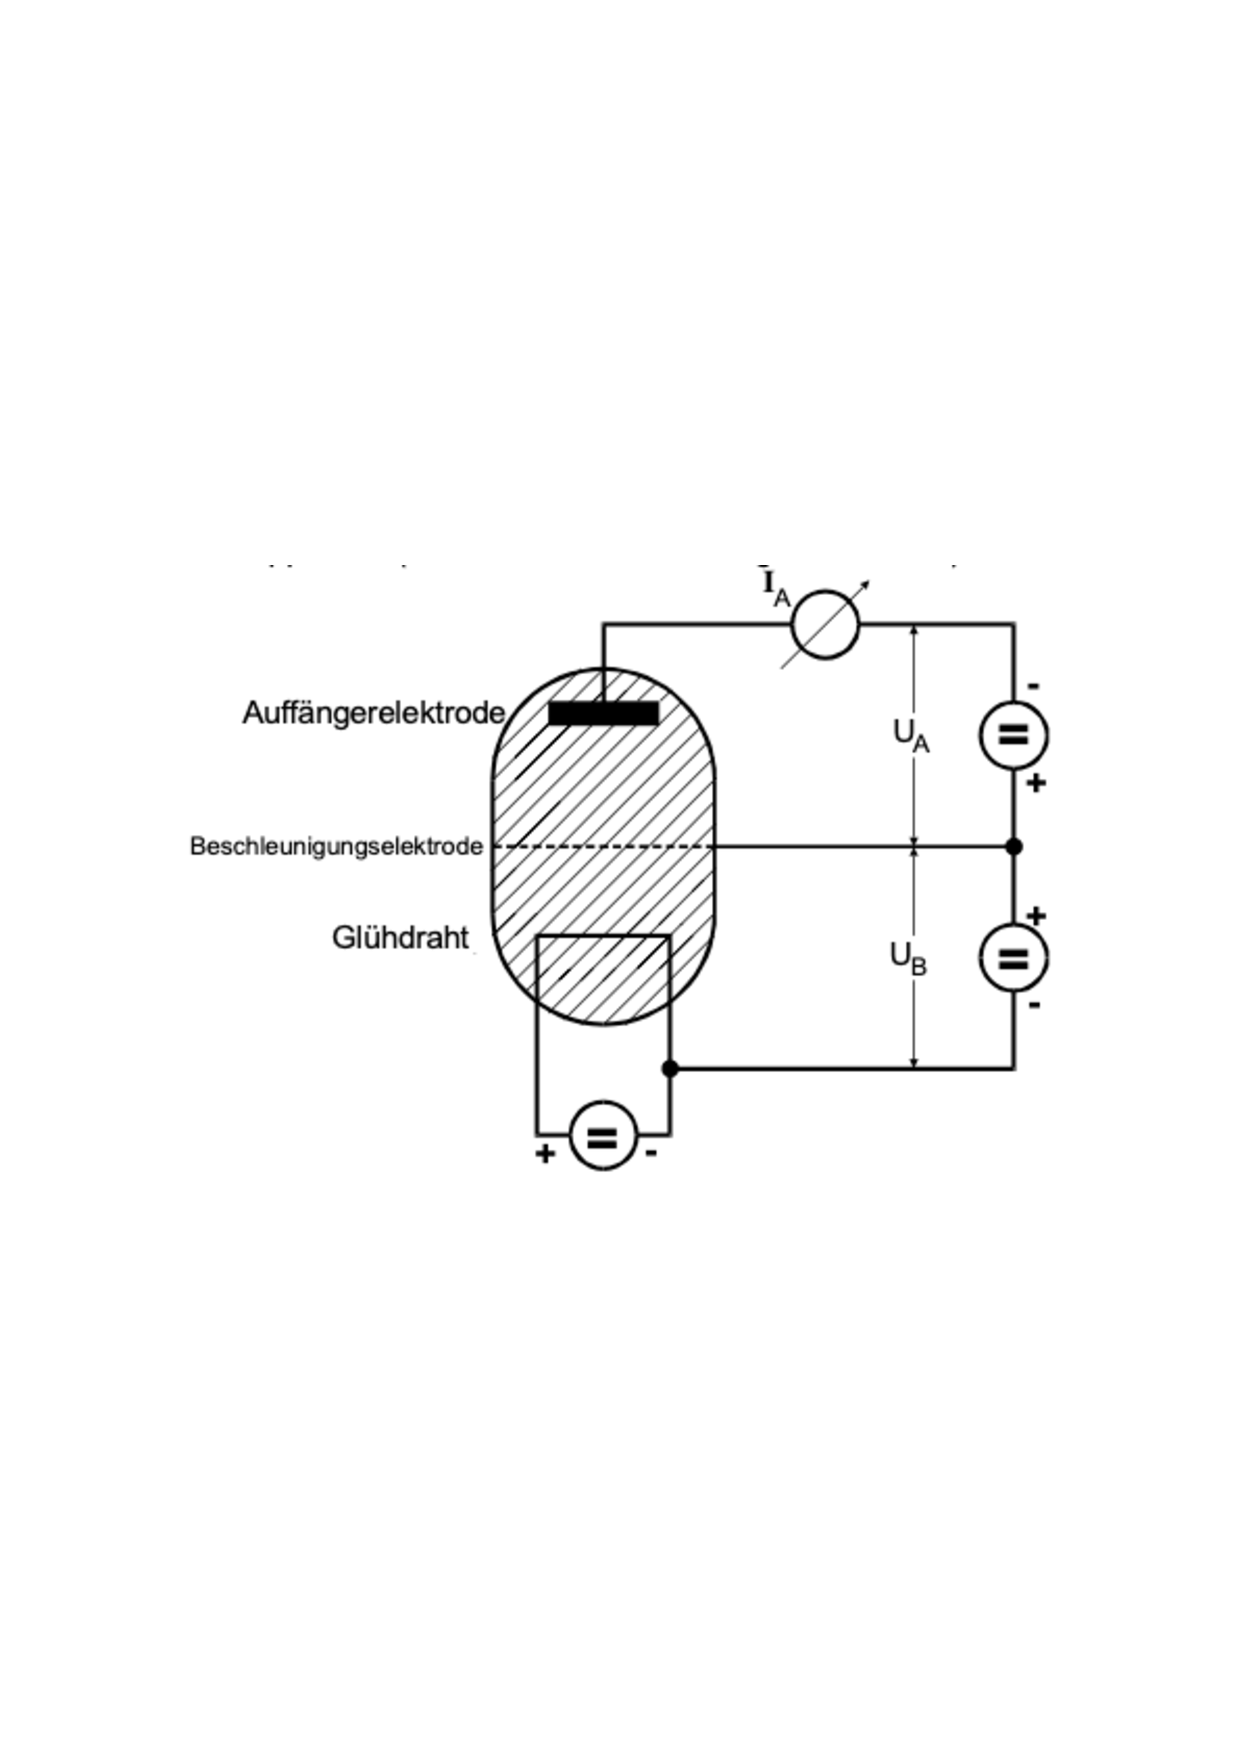
\includegraphics[height=6cm]{content/pics/FH-Aufbau.pdf}
    \caption{Aufbau einer Franck-Hertz-Röhre.\cite{v601}}
    \label{fig:Aufbau}
\end{figure}
Dafür wird eine Heizspannung an einer Glühkathode angelegt, wodurch Elektronen aufgrund des glühelektrischen Effekts austreten.
Diese Elektronen werden mit einer Beschleunigungsspannung $U_{\symup{B}}$ zu der Beschleunigungsanode hin beschleunigt.
Dabei kommt es zu den in \ref{sec:Anregung} beschriebenen Stößen zwischen den Elektronen und den Hg-Atomen. Die Energie der Elektronen 
nach den Stößen wird mithilfe der Gegenfeldmethode bestimmt. Demnach gilt für die kinetische Energie der Elektronen
\begin{equation}
    \frac{m_{\symup{e}}v^2}{2}≥eU_{\symup{A}}
    \label{eq:E-kin}
\end{equation}
wobei hier $U_{\symup{A}}$ die Bremsspannung beschreibt. Dies ergibt sich aus der Tatsache, dass nur Elektronen mit hinreichend großer
kinetischer Energie die Auffangelektrode erreichen.

Die Elektronen können bei großer Beschleunigungsspannung nach einem Stoß erneut beschleunigt werden, sodass sich der Strom an der
Auffangelektrode idealerweise wie in \autoref{fig:FH-Ideal} verhält.

\begin{figure}[H]
    \centering
    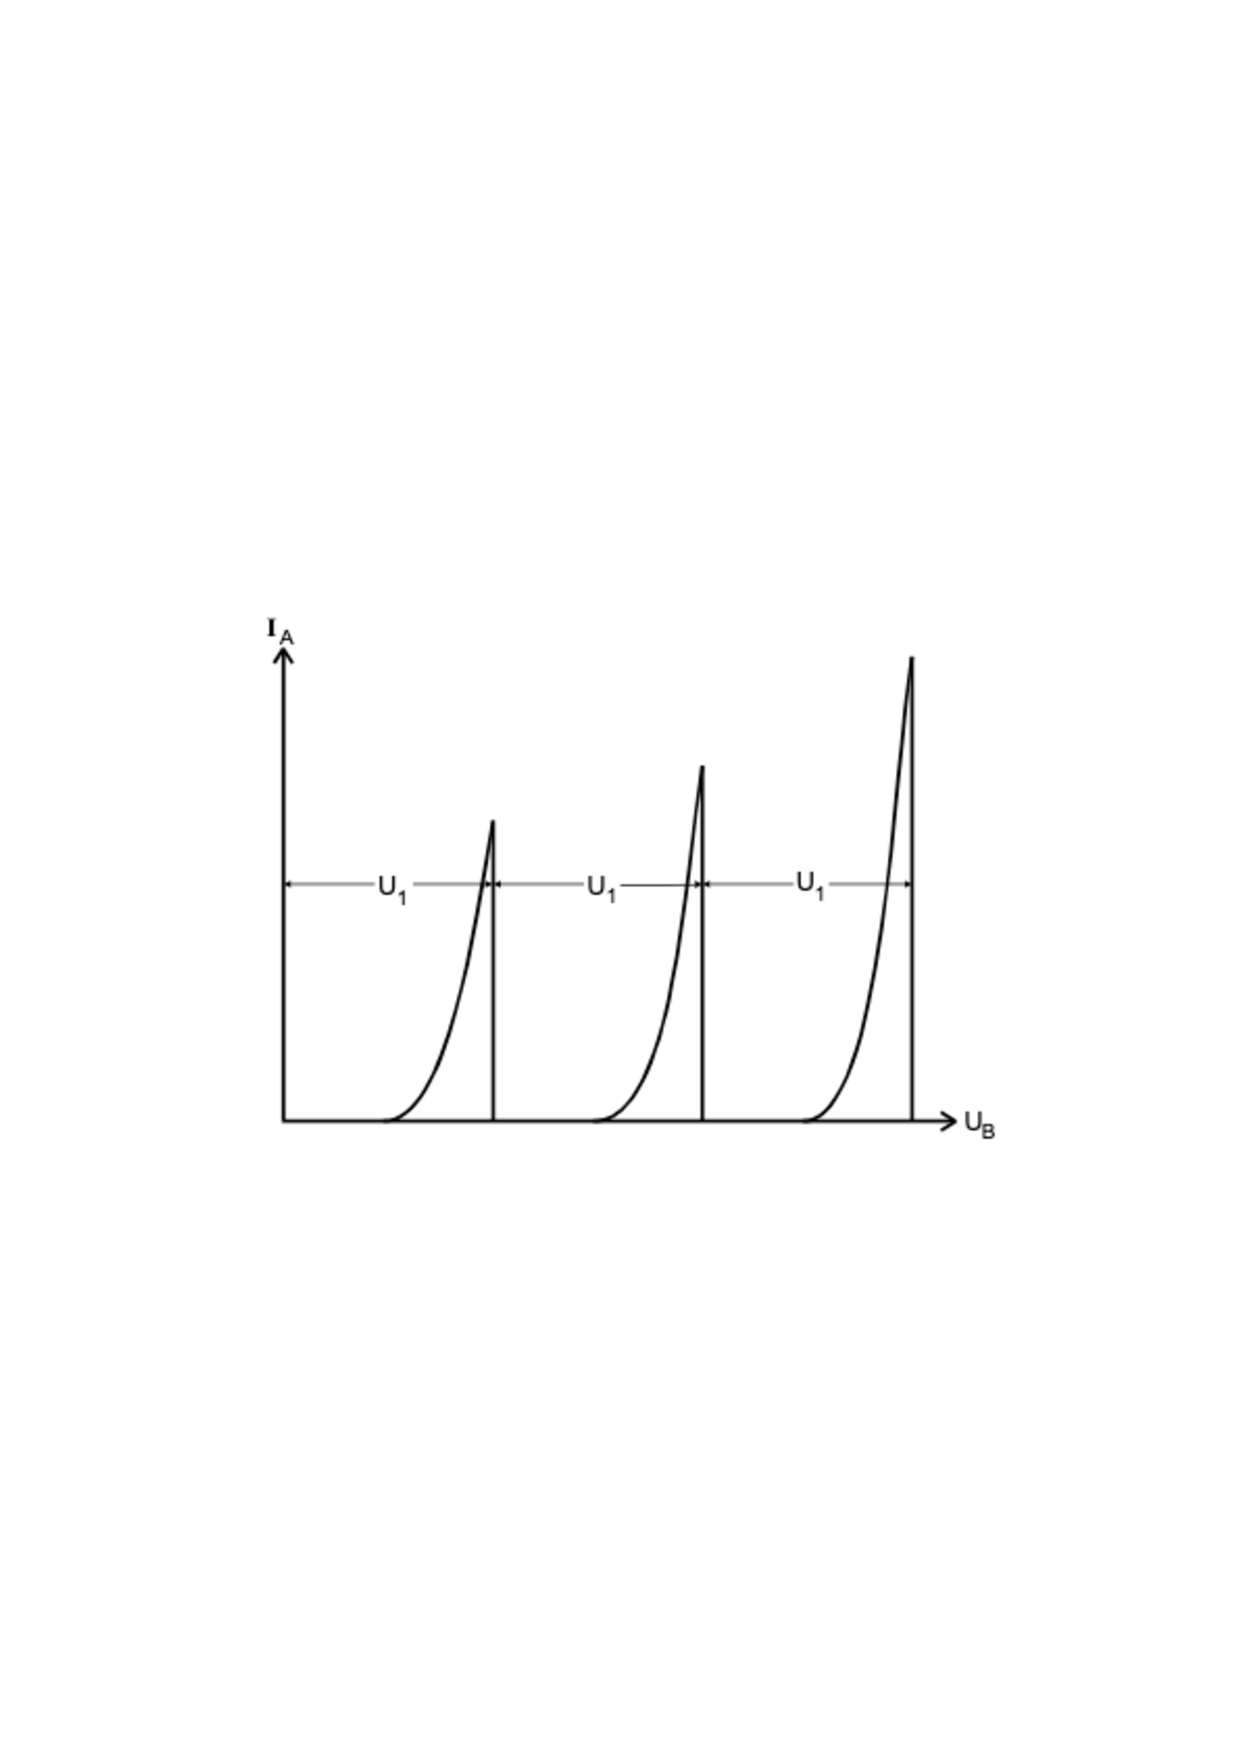
\includegraphics[height=6cm]{content/pics/FH-Ideal.pdf}
    \caption{Idealisierte Franck-Hertz-Kurve.\cite{v601}}
    \label{fig:FH-Ideal}
\end{figure}

\subsection{Störeffekte}
\label{sec:Störeffekte}
Aufgrund experimenteller Beschränkungen weicht die tatsächlich zu beobachtende Franck-Hertz-Kurve von der idealisierten ab. 
Gründe und deren Effekte dafür werden im Folgenden aufgeführt.

\subsubsection{Kontaktpotential}
In der zu verwendenden Franck-Hertz-Röhre werden für die Glüh- und die Auffangelektrode unterschiedliche Materialien verwendet. 
Dadurch ist das Fermi-Potential zwischen den Materialien nicht ausgeglichen, was zu einer Veränderung der tatsächlichen 
Beschleunigungsspannung führt. Daher ist die Franck-Hertz-Kurve verschoben und die Effektivspannung entspricht nicht der 
Beschleunigungsspannung, sie lässt sich über die Differenz
\begin{equation}
    U_{\symup{eff}} = U_{\symup{B}} - K
    \label{eq:Kontaktpotential}
\end{equation}
ausrechnen.

\subsubsection{Energiespektrum der Elektronen}
Die aus der Glühkathode austretenden Elektronen sind nicht monoenergetisch, da sie bereits im Inneren der Kathode ein Energiespektrum 
besitzen. Folglich weist die Franck-Hertz-Kurve keine diskreten Peaks auf und ist stattdessen abgeflacht und verbreitert.

\subsubsection{Dampfdruck}
Die Atome in der Franck-Hertz-Röhre müssen eine mittlere freie Weglänge $\bar{w}$ haben, die klein gegenüber dem Abstand zwischen 
der Glüh- und der Auffangelektrode ist, damit viele Stöße zwischen Elektronen und Hg-Atomen auftreten.

Die freie Weglänge $\bar{w}$ lässt sich über den Dampfdruck regulieren, welcher wiederum durch die Temperatur $T$ gegeben 
ist. Aus der kinetischen Gastheorie folgt der Zusammenhang
\begin{align}
    \bar{w}(T) &= \frac{0,0029}{\num{5.5e7} \symup{e}^{\frac{-6876}{T}}}. & [\bar{w}] &= \unit{\centi\metre} \label{eq:freie weglänge} %\\
     %{}& [T] &= \unit{\kelvin} \notag
\end{align}

Es ergibt sich, dass die Wahrscheinlichkeit für die erwünschten unelastischen Stöße für eine bestimmten Temperaturbereich optimal ist. Ist 
die Temperatur gering, ist auch die Stoßwahrscheinlichkeit niedrig. Im Fall einer hohen Temperatur kommt es vemehrt zu elastischen Stößen 
und somit zu keiner Anregung der Hg-Atome.